\documentclass[9pt, a4paper, notitlepage]{extreport}
\usepackage{kactlpkg}
\usepackage[nodisplayskipstretch]{setspace}
\usepackage{kotex}
\usepackage{physics}
\usepackage{float}
\kactlcontentdir{content}

\university{SNU}{Seoul National University}{}
\team{Jaechan Lee}{Jaechan Lee}
\contest{LGCPC}{September, 2024}
% \enablecolors

\begin{document}
	\maketeampage
	%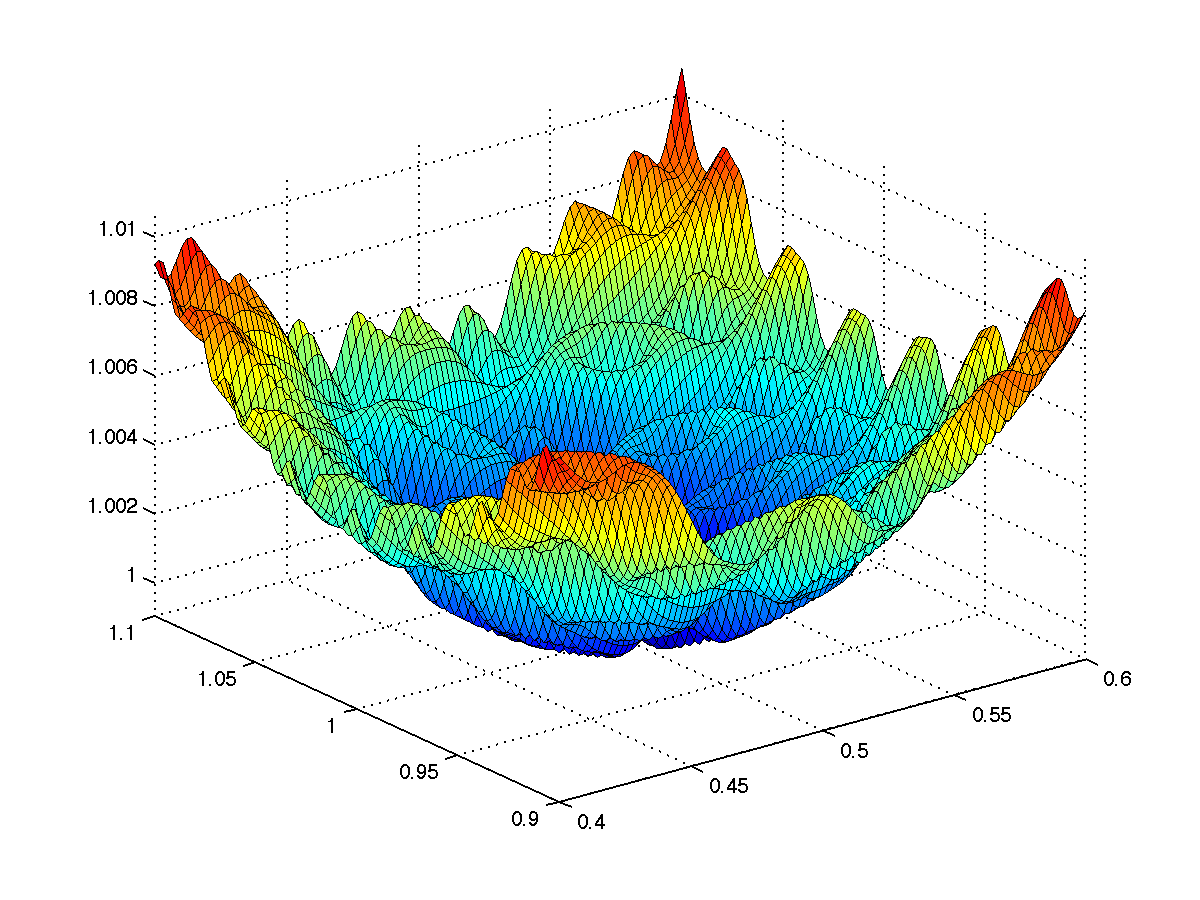
\includegraphics{content/tex/cover.png}
	% Small KACTL header on the first page:
	% \maketitle{``One Last Time'' Edition}{\today}
	\begin{multicols*}{3}
	\thispagestyle{fancy}
	% Table of contents, without subsections:
	\setcounter{tocdepth}{1}
	\tableofcontents

	\kactlchapter{data-structures}
	\kactlchapter{math}
	\kactlchapter{number-theory}
	\kactlchapter{numerical}
	\kactlchapter{combinatorics}
	\kactlchapter{graph}
	\kactlchapter{geometry}
	\kactlchapter{strings}
	\kactlchapter{dp-opt}
	\kactlchapter{various}
	\end{multicols*}

	\begin{multicols*}{2}
	\chapter{Checkpoints}
	\section{Debugging}
	\begin{itemize}
	  \item $10^5 * 10^5 \Rightarrow \text{OVERFLOW}$. 특히 for 문 안에서 \texttt{i * i < n} 할때 조심하기.
	  \item If unsure with overflow, use \\
	  \texttt{\#define int long long} and stop caring.
	  \item 행렬과 기하의 $i, j$ 인덱스 조심. 헷갈리면 쓰면서 가기.
	  \item 행렬에서는 $(r, c)$, 기하에서는 $(x, y)$ 로 문제를 표현하는 것이 많은 도움이 된다.
	  \item Segment Tree, Trie, Fenwick 등 Struct 구현체 사용할 때는 항상 내부의 $n$ 이 제대로 초기화되었는지 확인하기.
	  \item Testcase가 여러 개인 문제는 항상 초기화 문제를 확인하기. 입력을 다 받지 않았는데 break나 return으로 끊어버리면 안됨.
	  \item iterator 주의 : .end() 는 항상 맨 끝 원소보다 하나 더 뒤의 iterator. erase쓸 때는 iterator++ 관련된 문제들에 주의.
	  \item std::sort must compare with Strict weak ordering \textcolor{red}{(Codejam 2020 1A-A)}
	  \item Memory Limit : Local variable은 int 10만개 정도까지만 사용. Global Variable의 경우 128MB면 대략 int 2000만 개까지는 잘 들어간다. long long은 절반. stack, queue, map, set 같은 특이한 컨테이너는 100만개를 잡으면 메모리가 버겁지만 vector 100만개는 잡아도 된다.
	  \item Array out of Bound : 배열의 길이는 충분한가? Vector resize를 했다면 그것도 충분할까? 배열의 -1번에 접근한 적은 없는게 확실할까?
	  \item Binary Search : 제대로 짠 게 맞을까? 1 차이 날 때 / lo == hi 일 때 등등. Infinite loop 주의하기.
	  \item Graph : 반례 유의하기. Connected라는 말이 없으면 Disconnected. Acyclic 하다는 말이 없으면 Cycle 넣기, 특히 $A \leftrightarrow B$ 그래프로 2개짜리 사이클 생각하기.
	\end{itemize}
	\section{Thinking}
	\begin{itemize}
		\item 모든 경우를 다 할 수 없나? 왜 안 되지? 시간 복잡도 잘 생각해 보기. 정해의 Target Complexity를 먼저 생각하고 주요 알고리즘들의 Complexity로 짜맞추기.\\
		예를들어, 쿼리가 30만개 들어온다면 한 쿼리를 적어도 $\log{n}$ 에 처리할 방법이 아무튼 있다는 뜻.
        \item 보다 쉬운 문제를 풀기. ``$N$이 얼마 정도로 작다면...''
        \item 보다 특수한 문제를 풀기. ``만약 쿼리가 정렬되어 있다면...'', ``만약 주어진 그래프가 트리 형태라면...''
        \item STRANGE THINGS ARE IMPORTANT
		\item 그 방법이 뭐지? xxxx한 일을 어떤 시간복잡도에 실행하는 적절한 자료구조가 있다면?
		\begin{itemize}
			\item 필요한 게 정렬성이라면 힙이나 map을 쓸 수 있고
			\item multiset / multimap도 사용할 수 있고.. 느리지만.
		\end{itemize}
		\item 단조함수이며, 충분히 빠르게 검증가능한가 : Binary Search.
		\item 차원이 높은 문제 : 차원 내려서 생각하기. 3 $\rightarrow$ 2. 2 $\rightarrow$ 1. \textcolor{red}{2019 Codejam R1B-1 Manhattaen Crepe Cart}
		\item 이 문제가 사실 그래프 관련 문제는 아닐까?
			\begin{itemize}
				\item 만약 그렇다면, `간선' 과 `정점' 은 각각..?
				\item 간선과 정점이 몇 개 정도 있는가?
			\end{itemize}
		\item 이 문제에 Overlapping Subproblem이 보이나? \\$\rightarrow$ Dynamic Programming 을 적용.
		\item Directed Graph, 특히 Cycle에 관한 문제 : Topological Sorting? \textcolor{red}{(ex : SNUPC 2019 kdh9949)}
		\item 일반적인 directed graph를 다루기는 상당히 까다롭다. 항상 SCC + DAG를 생각하기. 
		\item 답의 상한이 Reasonable 하게 작은가? 
		\item output이 특정 수열/OX 형태 : 작은 예제를 Exhasutive Search. 모르는 무언가를 알기 위해서는 데이터가 필요하다.
		\item 그래프 문제에서, 어떤 ``조건" 이 들어갔을 때 $\to$ 이 문제를 ``정점을 늘림으로써" 단순한 그래프 문제로 바꿀 수 있나? (ex : SNUPC 2018 달빛 여우) 이를테면, 홀짝성에 따라 점을 2배로 늘림으로써?
		\item DP도 마찬가지. 어떤 조건을 단순화하기 위해 상태의 수를 사이사이에 집어넣을 수 있나? (ex : SNUPC 2018 실버런)
		\item DP State를 어떻게 나타낼 것인가? 첫 $i$개만을 이용한 답을 알면 $i+1$개째가 들어왔을 때 빠르게 처리할 수 있을까?
		\item 더 큰 table에서 시작해서 줄여가기. 특히 Memory가 모자라다면 Toggling으로 차원 하나 내릴 수 있는 경우도 상당히 많이 있다. 각 칸의 갱신 시간과 칸의 개수 찾기.
		\item Square root Decomposition : $O(n \log n)$ 이 생각나면 좋을 것 같지만 잘 생각나지 않고, 제한을 보니 $O(n \sqrt{n})$ 이면 될것도 같이 생겼을 때 생각해 보기. $O(\sqrt{n})$ 버킷 테크닉. \textcolor{red}{Red Army 2020 : Queue}
		\item 복잡도가 맞는데 왜인지 안 뚫리면 : 필요없는 long long을 사용하지 않았나? map이나 set iterator들을 보면서 상수 커팅. 간단한 함수들을 inlining. 재귀를 반복문으로. Set과 Map.
		\item 마지막 생각 : 조금 추하지만 해싱이나 Random 또는 \texttt{bitset} 을 이용한 $n^2 / 64$ 같은걸로 뚫을 수 있나? 컴파일러를 믿고 $10^8$의 몇 배 정도까지는 내 봐도 될 수도. 의외로 Naive한 문제가 많다. \textcolor{red}{Atcoder 158 Divisible Substring}
	\end{itemize}

		\end{multicols*}

\end{document}
